\documentclass[]{article}

% Imports the catppuccin theme, using the mocha flavor,
% from the directory above. Actual implementation
% wouldn't need the import package unless the theme
% and the document are in different directories.
\usepackage{import}
\usepackage{xcolor}
% \usepackage{fancyhdr}
\usepackage{cancel}
\usepackage{mathtools}

% For permutations and combinations
\newcommand\Myperm[2][^n]{\prescript{#1\mkern-2.5mu}{}P_{#2}}
\newcommand\Mycomb[2]{\prescript{#1\mkern-0.5mu}{}C_{#2}}

% Colors
\definecolor{yorhabg}{HTML}{FFFFFF}
\definecolor{yorhafg}{HTML}{000000}
\definecolor{yorhagrid}{HTML}{B5AF9C}
\definecolor{mred}{HTML}{D67069}
\definecolor{mblue}{HTML}{6887A1}

\pagecolor{yorhabg}
\color{yorhafg}

\usepackage{preamble}

% Removes padding above title
\usepackage{titling}
\setlength{\droptitle}{-10em}

% Font package
\usepackage[T1]{fontenc}

\usepackage{fouriernc}

\usepackage{sectsty}
\usepackage{graphicx}
\usepackage{amsmath}
\usepackage{amsfonts}
\usepackage{amssymb}
\usepackage[skins, most]{tcolorbox}
\usepackage{enumitem}

\DeclareMathOperator{\sgn}{sgn}

\usepackage{tikz}
\usepackage{eso-pic}
\usetikzlibrary{calc,shadows.blur}
\usetikzlibrary{angles, quotes}
\usetikzlibrary{3d}

% Margins
\topmargin=0in
\evensidemargin=0in
\oddsidemargin=0in
\textwidth=6.5in
\textheight=9.0in
\headsep=0.25in

\AtBeginEnvironment{tcolorbox}{\small}

\newtcolorbox{imp}{enhanced,arc=0mm,colback=yorhabg,colframe=mred,leftrule=10mm,coltext=yorhafg,%
overlay={\node[anchor=west,outer sep=2pt] at (frame.west) {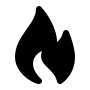
\includegraphics[width=6mm]{images/imageb.png}}; }}

\newtcolorbox{shortcut}{enhanced,arc=0mm,colback=yorhabg,colframe=mred,leftrule=10mm,coltext=yorhafg, coltitle=yorhabg, title=\texttt{Shortcut.}, 
overlay={\node[anchor=west,outer sep=2pt] at (frame.west) {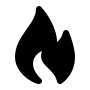
\includegraphics[width=6mm]{images/imageb.png}}; }}

\newtcolorbox{question}[1]{
    enhanced, 
    colback=yorhabg,
    colframe=mblue,
    coltext=yorhafg,
    coltitle=yorhabg,
    attach boxed title to top left={yshift*=-\tcboxedtitleheight}, 
    title=\texttt{#1},
    boxed title size=title,
    boxed title style={%
        rounded corners=northeast, 
        rounded corners=northwest, 
        colback=tcbcolframe, 
        boxrule=0pt,
    },
    underlay boxed title={%
        \path[fill=tcbcolframe] (title.south west)--(title.south east) 
            to[out=0, in=180] ([xshift=5mm]title.east)--
            (title.center-|frame.east)
            [rounded corners=5pt] |- 
            (frame.north) -| cycle; 
    },
}

\newcommand\bb[1]{\textcolor{yorhafg}{\textbf{#1}}}

\title{\textbf{CSCA67 - Exercises \#6}}
\author{Satyajit Datta \ 1012033336}
\date{\today}

\begin{document}

\maketitle

For each of the following arguments, either prove the argument is valid by using Inference Rules or
prove the argument is invalid by providing a counter-example world.

\begin{question}{1.1}
    All birds eat at least one species of insect. All species of insects can fly. Therefore, all birds eat at
    least one flying species.

    Let $I(x)$ be “$x$ is a species of insect”, $B(x)$ be “$x$ is a bird”, $F(x)$ be “$x$ flies”, and $E(x, y)$ be
    “$x$ eats $y$”. Universe of discourse is live beings.
\end{question}



\begin{flalign*}
    &\forall x,\; B(x) \rightarrow (\exists y, I(y) \land E(x, y)) && (1) \\
    &\forall x,\; I(x) \rightarrow F(x) && (2) \\
    &\forall x,\; B(x) \rightarrow (\exists y, F(y) \land E(x, y)) && \text{(Conclusion)}\\ 
    &\text{Take an arbitrary being }\; c && (3) \\
    &\quad B(c) \rightarrow (\exists y, I(y) \land E(c, y)) && (4) \ \text{(1,3, U.I)}\\ 
    &\quad \text{Suppose } B(c) && (5)\\ 
    &\quad\quad \exists y, I(y) \land E(c, y) && (5)\ \text{(3,4, Implication)}\\ 
    &\quad\quad \text{Choose d such that } I(d) \land E(c, d) && (6) \\
    &\quad\quad\quad I(d) \land E(c, d) && (7)\ \text{(5, E.I)}\\ 
    &\quad\quad\quad I(d) && (8)\ \text{(7, Simp.)}\\ 
    &\quad\quad\quad F(d) && (9)\ \text{(2, 8, U.M.P)}\\
    &\quad\quad\quad E(c, d) && (10)\ \text{(7, Simp.)}\\
    &\quad\quad\quad F(d) \land E(c, d) && (11)\ \text{(9, 10, Conj.)}\\
    &\quad\quad \exists y, F(y) \land E(c, y) && (12)\ \text{(6, 11, E.G)}\\
    &\quad B(c) \rightarrow (\exists y, F(y) \land E(c, y)) && (13) \ \text{(5, 12, Implication)}\\
    &\forall x,\; B(x) \rightarrow (\exists y, F(y) \land E(x, y)) && (14)\ \text{(3, 13, U.G)}\\ 
\end{flalign*} 

\begin{center}
    Therefore the argument is valid. $\blacksquare$
\end{center}

\begin{question}{1.2}
  Some smart people make lots of money. Some people who make lots of money buy very big houses.
Therefore, some smart people buy very big houses.

Let $S(x)$ stand for “$x$ is smart”, $M(x)$ be “$x$ makes lots of money”, and $H(x)$ be “$x$ buys a big
houses”, universe of discourse is people.
\end{question}

The argument given is:
\begin{align*}
    & \exists x\; S(x) \land M(x) & (1)\\
    & \exists x, M(x) \land H(x) & (2)\\
    & \overline{\exists x, S(x) \land H(x)} & \text{(Conclusion)}
\end{align*}
\vspace{0.1in}
Let $W \subseteq U$ s.t. $W = \{a, b, c\}$
\[
\begin{array}{c|c|c}
    \underline{a} & \underline{b} & \underline{c} \\ \hline
    S(a) = \text{True} & S(b) = \text{False} & S(c) = \text{True} \\
    M(a) = \text{True} & M(b) = \text{True} & M(c) = \text{False} \\
    H(a) = \text{False} & H(b) = \text{True} & H(c) = \text{False} \\
\end{array}
\]

\underline{\textbf{Premise (1)}}  
\[
\exists x, S(x) \land M(x)
\]
\begin{align*}
    &\text{Let } x = a \\
    &S(a) \land M(a) \\
    &T \land T \\
    &\textbf{T}
\end{align*}


\underline{\textbf{Premise (2)}}  
\[
\exists x, M(x) \land H(x)
\]
\begin{align*}
    &\text{Let $x = b$:} \\
    &M(b) \land H(b) \\
    &T \land T \\
    &\textbf{T}
\end{align*}


\underline{\textbf{Conclusion}}  
\[
\exists x, S(x) \land H(x)
\]
\begin{align*}
    &\text{Let $x = c$:} \\
    &S(c) \land H(c) \\
    &T \land F \\
    &\textbf{F}
\end{align*}

\hrule
\vspace{0.1in}
Thus, we have proved that there is a case such that all the premises are true, 
while the conclusion is false, making this argument invalid. $\blacksquare$


\begin{question}{1.3}
   Everybody knows at least one song. Every song is sung by someone. People only sing songs they
   like. Therefore, everyone knows at least one song someone likes.

    Let $S(x)$ be “$x$ is a song”, $P(x)$ be “$x$ is a person”, $K(x, y)$ be “$x$ knows $y$”, $L(x, y)$ be “$x$ likes
    $y$”, $S(x, y)$ be “$x$ sings $y$”. Universe of discourse is people and songs.
\end{question}

\begin{flalign*}
    &\forall x,\; P(x) \rightarrow (\exists y, S(y) \land K(x, y)) && (1) \\
    &\forall x,\; S(x) \rightarrow (\exists y, P(y) \land S(y, x)) && (2) \\
    &\forall x\forall y,\; (P(x) \land S(y) \land S(x, y)) \rightarrow L(x, y) && (3) \\
    &\forall x, P(x) \rightarrow (\exists y, S(y) \land K(x, y) \land \exists z, (P(z) \land L(z, y))) && \text{(Conclusion)}\\ 
    &\text{Let a be arbitrary.} && (4) \\ 
    &\quad \text{Suppose } P(a) && (5)\\ 
    &\quad\quad \exists y, S(y) \land K(a, y) && (6)\ \text{(1,5, Implication)}\\ 
    &\quad\quad \text{Choose b such that } S(b) \land K(a, b) && (7) \\
    &\quad\quad\quad S(b) \land K(a, b) && (8)\ \text{(7, E.I)}\\ 
    &\quad\quad\quad S(b) && (9)\ \text{(8, Simp.)}\\ 
    &\quad\quad\quad K(a, b) && (10)\ \text{(8, Simp.)}\\ 
    &\quad\quad\quad \exists y, P(y) \land S(y, b) && (11)\ \text{(2, 9, U.M.P)}\\
    &\quad\quad\quad \text{Choose c such that }  P(c) \land S(c, b) && (12)\ \text{(2, 9, U.M.P)}\\ 
    &\quad\quad\quad\quad  P(c) \land S(c, b)&& (13)\ \text{(12, E.I)}\\ 
    &\quad\quad\quad\quad  S(b) \land P(c) \land S(c, b)&& (14)\ \text{(9, 13, Conj.)}\\ 
    &\quad\quad\quad\quad  L(c, b) && (15)\ \text{(3, 14, U.M.P)}\\ 
    &\quad\quad\quad\quad  P(c) && (16)\ \text{(13, Simp.)}\\ 
    &\quad\quad\quad\quad  P(c) \land L(c, b) && (17)\ \text{(15, 16, Conj.)}\\ 
    &\quad\quad\quad \exists z, P(z) \land L(z, b) && (18)\ \text{(17, 12, E.G)}\\ 
    &\quad\quad\quad S(b) \land K(a, b) \land (\exists z, P(z) \land L(z, b)) && (19)\ \text{(18, 8, conj.)}\\ 
    &\quad\quad \exists y, S(y) \land K(a, y) \land (\exists z, P(z) \land L(z, y)) && (20)\ \text{(19, 7, E.G)}\\ 
    &\quad P(a) \rightarrow (\exists y, S(y) \land K(a, y) \land (\exists z, P(z) \land L(z, y))) && (21)\ \text{(19, 7, Implication)}\\ 
    &\forall x, P(x) \rightarrow (\exists y, S(y) \land K(x, y) \land \exists z, (P(z) \land L(z, y))) && (22) \ \text{(4, 21, U.G)}\\   
\end{flalign*} 

\begin{center}
    Therefore the argument is valid. $\blacksquare$
\end{center}

\begin{question}{2.1}
   Prove: If x, y, and z are integers and x + y + z is odd, then at least one of x, y, z is odd
\end{question}
Universe of discourse is integers.
\[
    WTS: O(x + y + z) \rightarrow (O(x) \lor O(y) \lor O(z))
\]

\begin{center}
    Lemmas.
\end{center}
\[
    (**): E(x) \leftrightarrow \exists k, x = 2k 
\]
\[
    (***): \neg E(x) = O(x) 
\]
\begin{flalign*}
    &\text{Suppose } E(x) \land E(y) \land E(z) && (1) \\
    &\quad(\exists k, x=2k) \land (\exists j, y=2j) \land (\exists i, z=2i) && (2)\ \text{(1, (**))}\\
    &\quad x=2k && (3)\ \text{(2, E.I)}\\
    &\quad y=2j && (4)\ \text{(2, E.I)}\\
    &\quad z=2i && (5)\ \text{(2, E.I)}\\
    &\quad x+y+z = 2(k+j+i) && (6) \ \text{3, 4, 5, algebra} \\
    &\quad E(x+y+z) && (7)\ \text{(6, (**))} \\
    &(E(x) \land E(y) \land E(z)) \rightarrow E(x+y+z) && (8)\ \text{(1, 7, Implication)}\\
    &\neg E(x+y+z) \rightarrow \neg(E(x) \land E(y) \land E(z))&& (9)\ \text{(8, contra.)}\\
    &\neg E(x+y+z) \rightarrow (\neg E(x) \lor \neg E(y) \lor \neg E(z))&& (10)\ \text{(9, DeM.)}\\
    &O(x + y + z) \rightarrow (O(x) \lor O(y) \lor O(z)) && (11)\ \text{(10, (***))}\\
\end{flalign*}

\begin{question}{2.2}
   Prove: If $n$ is a positive integer, then $n$ is even if and only if $7n + 4$ is even.
\end{question}
Universe of discourse is $\mathbb{Z}^+$.

\[
    WTS: \forall n, E(n) \leftrightarrow E(7n+4) 
\]

\begin{center}
    Lemmas.
\end{center}
\[
    (*): O(x) \leftrightarrow \exists k, x = 2k+1 
\]
\[
    (**): E(x) \leftrightarrow \exists k, x = 2k 
\]
\[
    (***): \neg O(x) = E(x) 
\]
\begin{flalign*}
    &\text{Take an arbitrary positive integer } n && (1) \\
    &\quad \text{Suppose } E(n)  && (2) \\
    &\quad\quad \exists k, n = 2k && (3) \\
    &\quad\quad n = 2k && (4)\ \text{3, E.I} \\
    &\quad\quad 7n+4 = 7(2k) + 4 && (5)\ \text{4, algebra} \\
    &\quad\quad 7n+4 = 2(7k + 2) && (6)\ \text{5, algebra} \\
    &\quad\quad E(7n+4) && (7)\ \text{6, (**)} \\
    &\quad E(n) \rightarrow E(7n+4) && (8)\ \text{(2, 7, Implication)}\\
    &\quad \text{Assume } O(n) && (9)\\
    &\quad\quad \exists k, n = 2k+1 && (10)\ \text{(9, (*))}\\
    &\quad\quad n = 2k+1 && (11)\ \text{(10, E.I)}\\
    &\quad\quad 7n+4 = 7(2k+1) +4 && (12)\ \text{(11, algebra)}\\
    &\quad\quad 7n+4 = 14k+7+4 && (13)\ \text{(12, algebra)}\\
    &\quad\quad 7n+4 = 14k+11 && (14)\ \text{(13, algebra)}\\
    &\quad\quad 7n+4 = 2(7k+5)+1 && (15)\ \text{(14, algebra)}\\
    &\quad\quad O(7n+4) && (16)\ \text{(15, (*))}\\
    &\quad O(n) \rightarrow O(7n+4) && (17)\ \text{(9, 16, Implication)}\\
    &\quad \neg O(n) \rightarrow \neg O(7n+4) && (18)\ \text{(18, Contr.)}\\
    &\quad E(n) \rightarrow E(7n+4) && (19)\ \text{(18, (***))}\\
    &\quad (E(n) \rightarrow E(7n+4)) \land (E(n) \rightarrow E(7n+4)) && (20)\ \text{(8, 20, Conj.)}\\
    &\quad (E(n) \leftrightarrow E(7n+4)) && (21)\ \text{(20, bicond.)}\\
    &\forall n, E(n) \leftrightarrow E(7n+4) && (22) \ \text{(1, 20, U.G)}
\end{flalign*}


\begin{question}{2.3}
   Prove: $(A \cap B \ne \emptyset \; \land \; A \subseteq C) \rightarrow (B \cap C \ne \emptyset)$
\end{question}

\begin{flalign*}
    &\text{Suppose } A \cap B \ne \emptyset \land A \subseteq C && (1) \\
    &\quad\exists x (x \in A \land x \in B) && (2)\ \text{(1, Definition of $\cap$)}\\
    &\quad\text{Choose } x \text{ such that } x \in A \land x \in B && (3)\\
    &\quad\quad x \in A &&(4)\ \text{(3, Simp.)}\\
    &\quad\quad x \in B &&(5)\ \text{(3, Simp.)} \\
    &\quad\quad \forall y (y \in A \rightarrow y \in C) &&(6)\ \text{(definition of $\subseteq$)} \\
    &\quad\quad x \in C && (7)\ \text{(4,6, U.M.P)} \\
    &\quad\quad x \in B \land x \in C &&(8)\ \text{(5,7, Conj.)} \\
    &\quad\exists x (x \in B \land x \in C) &&(9)\ \text{(3,8, E.G)}\\
    &\quad B \cap C \ne \emptyset &&(10) \text{(9, definition of $\cap$)}\\
    &(A \cap B \ne \emptyset \; \land \; A \subseteq C) \rightarrow (B \cap C \ne \emptyset) &&(11) \text{(1, 10, Implication)}
\end{flalign*}

\begin{center}
\(\therefore\) As required to show. \(\blacksquare\)
\end{center}
\end{document}